\documentclass[handout]{beamer}

\usepackage{tikz}
\usetikzlibrary{arrows,shapes,positioning,shadows,trees}
\usepackage{graphicx}
\usepackage{multimedia}
\usepackage[latin1]{inputenc}
\usecolortheme{lily}
\setbeamercovered{transparent}

\title[\insertdate]{Nonparametric Bayes}

\author{Omar Guti\'errez}
\institute{@omargtz}
\date{June 15, 2015}

\begin{document}

\begin{frame}
\titlepage
Mostly based on \textbf{A Tutorial on Bayesian Nonparametric Models} by Samuel J. Gershman.
\end{frame}

\section{The Intuition Behind}
\begin{frame}{Let's think in the next cases}
    \begin{itemize}
        \item The articles in Wikipedia
        \item The species in the planet
        \item The hashtags on Twitter
    \end{itemize}
\end{frame}

\begin{frame}{Intuition}
    \begin{itemize}
        \item How many classes should I use in my mixture model?
        \item How many factors should I use in factor analysis?
        %\item Learning more from the data as we see it.
        %\item Non-parametric models have infinite number $\theta$ parameters.
        %\item Examples, topics in Wikipedia, species, social networks
    \end{itemize}
\end{frame}

\section{Clustering}
\begin{frame}{Clustering}
	\begin{itemize}
        \item Let's consider the clustering
        \item We want to get $k$ clusters
        \item We can use Gaussian Mixture Models
	        \begin{itemize}
                \item We learn the parameters of the Gaussians:
	        \end{itemize}
        \item $ \mu_{k} \overset{iid}{\sim} \mathcal{N}(\mu, \sigma^{2}) $
        \item We can use techniques to evaluate the best clustering, e.g. Silhuotte, and then decide using cross-validation.
        \item Another interesting approach is to use Bayesian Nonparametric (BNP) models
        \item BNP models will build a model than can adapt its complexity to the data
        % Put an image with clusters here.
	\end{itemize}
\end{frame}

\begin{frame}{Bayesian parametric vs nonparametric models}
    \begin{itemize}
        \item Traditional approach (finite)
           \begin{itemize}
               \item The number of parameters $\theta$ (e.g. clusters) is prespecified
               \item We have a prior distribution over parameters $P(\theta)$
               \item For example, in the Gaussian mixture model, each cluster will be modelled
                   using a parametric model (e. g. Gaussian)
           \end{itemize}
        \item Bayesian nonparametric models
           \begin{itemize}
               \item We assume that there is an \textbf{infinite} number of latent clusters
               \item A finite number of clusters is \textit{inferred} from data
               \item The number of clusters grow as new data points are observed
           \end{itemize}
    \end{itemize}
\end{frame}

\section{Bayesian nonparametric models}
\begin{frame}{Bayesian nonparametric models}

    \begin{figure}[H]
        \centering
        \tikzset{
  basic/.style  = {draw, text width=2cm, align=center, drop shadow, font=\sffamily\footnotesize, rectangle, fill=gray!30},
  root/.style   = {basic, rounded corners=2pt, thin},
  level 2/.style = {basic, rounded corners=6pt, thin, text width=6em},
  level 3/.style = {basic, rounded corners=2pt, thin, text width=5em},
  level 4/.style = {basic, rounded corners=2pt, thin, text width=6em, font=\tiny}
}

\begin{tikzpicture}[
  level 1/.style={sibling distance=40mm},
  edge from parent/.style={->,draw},
  edge from node/.style={->,draw, black},
  >=latex]

% root of the the initial tree, level 1
\node[root] {\textbf{Bayesian models}}
% The first level, as children of the initial tree
  child {node[level 2] (c1) {Parametric}}
  child {node[level 2] (c2) {\textbf{Nonparametric}}
    child {node[level 3] (c21) {\textbf{Mixture}}
        child {node[level 4] (c211) {\textbf{Chinese Restaurant\\ Process}}}
    }
    child {node[level 3] (c22) {Latent factor}
        child {node[level 4] (c221) {Indian Buffet\\ Process}}
    }
  };

\node (comment) [above left = of c1] {Finite};
    \draw [->, thick] (comment) to [in = 110] (c1);

\node (comment2) [above right = of c2] {Infinite};
    \draw [->, thick] (comment2) to [in = 110] (c2);

\node (comment2) [above right = of c2] {Infinite};
    \draw [->, thick] (comment2) to [in = 110] (c2);

\node (comment3) [below left = of c211] {Dirichlet Processes!};
    \draw [->, thick] (comment3) to [in = 211] (c211);
    \draw [->, thick] (comment3) to [in = 221] (c221);

\end{tikzpicture}

    \end{figure}

\end{frame}

\section{Chinese Process Restaurant}
\begin{frame}{Chinese Restaurant Process}
    {\centering
    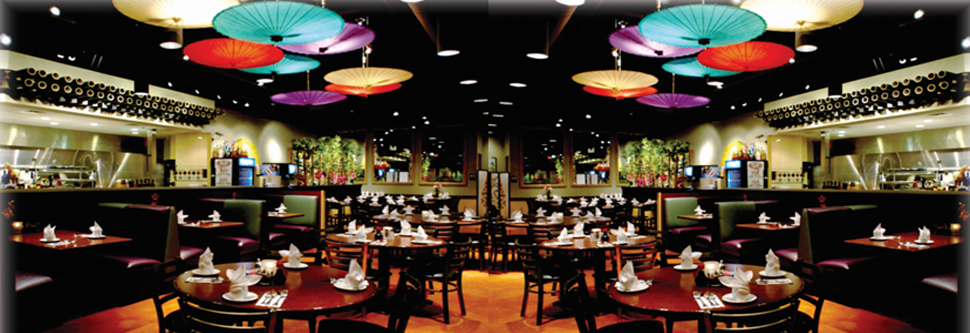
\includegraphics[width=0.75\textwidth]{figures/crp.png}\par
    }
    \pause

    \begin{itemize}
        \item Imagine a restaurant with an infinite number of tables,
        \item and a sequence of customers entering the restaurant and sitting down.
        \item The first customer enters and sits at the first table
        \item The second customer enters and sits...
            \begin{itemize}
                \item at the first table with probability $\frac{1}{1 + \alpha}$
                \item at the second table with probability $\frac{\alpha}{1 + \alpha}$
            \end{itemize}
        \item We realize that CRP is a form of clustering: $K$ groups and each group with size $N_k$
    \end{itemize}
\end{frame}

%\section{Bayesian Inference}
%\begin{frame}{Bayesian Inference}
%	\begin{itemize}
%        \item $P(A|D) \propto P(D|A) P(A)$
%	\end{itemize}
%\end{frame}

%\section{Generative Model}
%\begin{frame}{Generative Model}
%	\begin{itemize}
%        \item *
%	\end{itemize}
%\end{frame}


%\section{Python}
%\begin{frame}{Python}
%	\begin{itemize}
%        \item *
%	\end{itemize}
%\end{frame}

%\section{Beta and Dirichlet Distribution}
%\begin{frame}{Dirichlet Distribution}
%    \begin{itemize}
%        \item $\beta$ distribution.
%        \item Dirichlet distribution is a generalization of $\beta$ distribution.
%    \end{itemize}
%\end{frame}

\begin{frame}{What else?}
    \begin{itemize}
        %\item $\beta$ distribution.
        \item Dirichlet distribution is a generalization of $\beta$ distribution.
        \item Dirichlet process
    \end{itemize}
\end{frame}

\begin{frame}
\huge{Thank you}\\
\huge{Questions?}\\
\end{frame}

\end{document}
